\begin{figure*}[t]
	\centering
	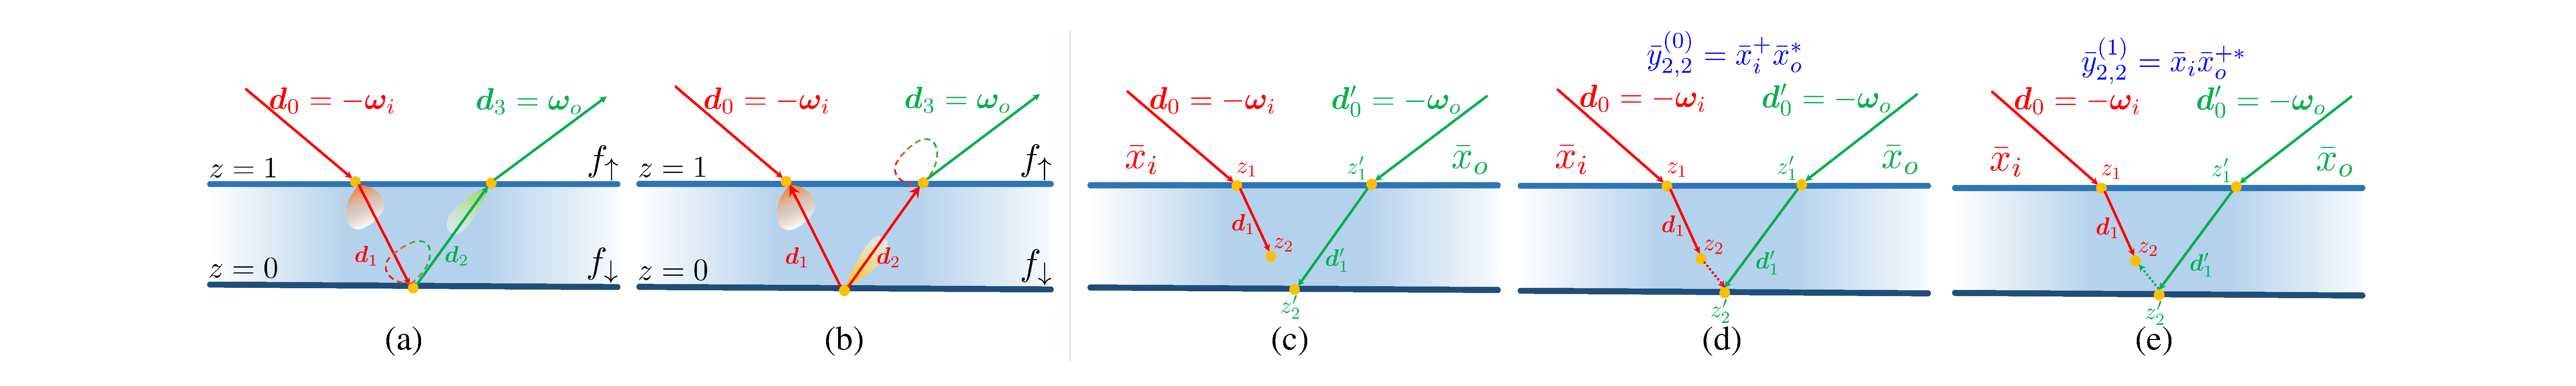
\includegraphics[width=\textwidth]{illustration/unidir-bidir.pdf}
	\caption{
		\label{fig:estimators}
		\textbf{Our Monte Carlo estimators} for BSDF values.
		\textbf{(ab)} Unidirectional estimator uses two path sampling strategies for ``shading'' a vertex on the bottom layer:
		(a)~sampling the BSDF $f_\uparrow$ of the top interface and connecting at the bottom (next event estimation); or (b)~sampling $\bd_2$ using $f_\downarrow$ and connecting at the top (path continuation). These strategies are combined using local MIS. \textbf{(cde)} Bidirectional estimator: (c) Two subpaths with initial directions $\omegain$ and $\omegaout$. (de) Two full light paths constructed by sampling an additional direction from each sub-path.
	}
\end{figure*}
